%! TeX program = lualatex
\documentclass[12pt]{article}

\usepackage{cmap}
\usepackage{newfloat}
\usepackage[newfloat]{minted}
\usepackage[font=small]{caption}
\usepackage{indentfirst}

\setminted{
    linenos,                % показывать номера строк
    breaklines,             % переносить длинные строки
    breakanywhere=true,     % переносить в любом месте
    tabsize=2,              % размер табуляции
    fontsize=\footnotesize,        % размер шрифта
    frame=lines,            % рамка сверху и снизу
    framesep=2mm,           % расстояние текста от рамки
    baselinestretch=1.1,    % межстрочный интервал
    autogobble=true,        % автоудаление общего отступа
    % xleftmargin=10pt,       % отступ слева
    % numbersep=5pt,          % расстояние между номерами и кодом
}

\usepackage[english, russian]{babel}

\usepackage[nopatch=footnote]{microtype}

\usepackage{float}
\usepackage{fontspec}
\usepackage[pdfborder={0 0 0}]{hyperref}

\usepackage{enumitem}

\makeatletter
\renewcommand\@seccntformat[1]{%
  \csname the#1\endcsname.\quad
}
\makeatother

\usepackage{tocloft}
\renewcommand{\cftsecaftersnum}{.}
\renewcommand{\cftsubsecaftersnum}{.}
\renewcommand{\cftsubsubsecaftersnum}{.}

\setmainfont{TimesNewerRoman}[
  Extension = .otf,
  Path = /nix/store/ihdqrn4p54awd89vrday9k53s8i47bbv-times-newer-roman-unstable-2018-09-11/share/fonts/opentype/,
  UprightFont = *-Regular,
  BoldFont = *-Bold
  ItalicFont = *-Italic
]
\setmonofont{Ubuntu Mono}

\newcommand{\icon}[1]{\fontspec{UbuntuNerdFont}[Extension = .ttf,
  Path = /nix/store/h721jafy2n74x4k5p0hxbz722h0rncmx-nerd-fonts-ubuntu-3.3.0+0.83/share/fonts/truetype/NerdFonts/Ubuntu/,
  UprightFont = *-Regular,
BoldFont = *-Bold] #1}

\newcommand{\iicon}[1]{{\icon{#1}}}

\usepackage{graphicx}
\usepackage{fontawesome5} % Для иконок

\usepackage[left=2.0cm, right=2.0cm, top=1.0cm, bottom=1.0cm, includeheadfoot]{geometry}

\usepackage[mocha, textcolor=true, pagecolor=true]{catppuccinpalette} \usemintedstyle{catppuccin-mocha}
% \usepackage[latte, textcolor=true, pagecolor=true]{catppuccinpalette} \usemintedstyle{catppuccin-latte}

\usepackage{setspace}
\onehalfspacing

\usepackage{fancyhdr}
\fancyhf{}

\renewcommand{\sectionmark}[1]{\markboth{#1}{}}
\renewcommand{\subsectionmark}[1]{\markright{#1}}

% Настройка колонтитулов
\fancyhead[RO]{\rightmark}
\fancyhead[LO]{\leftmark}

\fancyfoot[L]{\hspace{8pt} \rule{\textwidth}{0.4pt}}
\fancyfoot[R]{\LARGE{\thepage}}
\fancyfoot[C]{}

\newcommand{\lablogo}
{
\begin{center}
    \huge{\textbf{Лабораторная работа №5}} \\
\end{center}
}

\newcommand{\colorURL}[1]{\textcolor{CtpBlue}{#1}}
\newcommand{\colorGIT}[1]{\textcolor{CtpLavender}{#1}}
\renewcommand{\texttt}[1]{{\small\ttfamily #1}}

\setlength{\headheight}{15.2pt}

\DeclareCaptionLabelFormat{gostfigure}{Рисунок #2}
\captionsetup[figure]{labelformat=gostfigure, labelsep=endash}

\DeclareCaptionLabelFormat{gostlisting}{Листинг #2}
\newenvironment{code}{\captionsetup{type=listing}}{}
\captionsetup[listing]{labelformat=gostlisting, labelsep=endash}
% \DeclareFloatingEnvironment[
%   listname=Листинг,
% ]{listing}

\usepackage{amsmath}
\numberwithin{listing}{section}
\numberwithin{figure}{section}

\usepackage{tocloft}
\renewcommand{\cftsecleader}{\cftdotfill{\cftdotsep}}

\begin{document}
\pagestyle{empty}
\lablogo
\tableofcontents
\newpage
\listoflistings
\newpage

\pagestyle{fancy}

\section{Цель работы~\texorpdfstring{\iicon{}}{}}
Целью настоящей лабораторной работы является освоение базовых принципов создания REST\-ful-сервиса с применением технологии ASP.NET Core Web API и базы данных SQLite. В ходе выполнения работы осуществляется реализация функциональности добавления и получения информации о товарах, а также автоматическая генерация документации с использованием Swagger.

\noindent \textbf{Задание:}
\begin{enumerate}
	\item Изучить структуру ASP.NET Core Web API-проекта.
	\item Настроить Entity Framework Core и контекст базы данных.
	\item Создать модели и реализовать связи между ними.
	\item Реализовать контроллеры для управления товарами и заказами.
	\item Обеспечить создание базы данных при первом запуске.
\end{enumerate}

% \noindent Весь код доступен в \colorURL{\href{https://github.com/WebMasterIT/Csharp_Labs/tree/main}{репозитории на GitHub}\ \faGithub}\footnote{Ссылки, выделенные \colorURL{голубым} цветом, ведут на внешние ресурсы; ссылки, выделенные \colorGIT{светло-синим} цветом, указывают на исходный код в репозитории GitHub \ \faGithub. (Примечание: ссылка на репозиторий является общей для всех лабораторных работ, для данной работы актуальны файлы в соответствующей папке 5lab).}

\newpage

\section{Теоретические сведения~\texorpdfstring{\iicon{}}{}}
ASP.NET Core Web API представляет собой инфраструктуру для разработки HTTP-сервисов, архитектура которых основывается на контроллерах и маршрутах. Это позволяет обрабатывать REST-запросы и предоставлять данные в формате JSON.

\noindent \textbf{Ключевые технологии:}
\begin{itemize}
	\item ASP.NET Core
	\item Entity Framework Core
	\item SQLite
	\item REST
\end{itemize}

\noindent \textbf{Компоненты проекта:}
\begin{itemize}
	\item \texttt{Models} — классы бизнес-логики и структуры таблиц.
	\item \texttt{Data} — контекст базы данных.
	\item \texttt{Controllers} — обработка HTTP-запросов.
\end{itemize}

\pagebreak

\section{Порядок выполнения работы~\texorpdfstring{\iicon{󰈍}}{}}
В данном разделе последовательно описан процесс подготовки, запуска и анализа исходного кода проекта.

\subsection{Создание проекта}
Для начала необходимо выполнить следующие действия:
\begin{enumerate}
	\item В среде Visual Studio выбрать шаблон "ASP.NET Core Web API".
	\item Указать имя проекта: \texttt{StoreManagerApi}.
	\item При создании проекта активировать следующие опции:
	      \begin{itemize}
		      \item Controllers (включает шаблон контроллера);
		      \item Enable OpenAPI support (включает Swagger);
		      \item Enable HTTPS (в случае технических проблем допускается переключение на HTTP).
	      \end{itemize}
\end{enumerate}

\subsection{Структура проекта и назначение файлов}
Структура проекта выглядит следующим образом:
\begin{verbatim}
StoreManagerApi/
├── Controllers/
│   └── ProductController.cs // Обрабатывает HTTP-запросы, связанные с товарами
├── Data/
│   └── StoreDbContext.cs   // Представляет контекст базы данных SQLite
├── Models/
│   └── Product.cs     // Описывает модель данных для сущности "Товар"
├── Program.cs         // Конфигурирует сервисы и middleware приложения
├── appsettings.json  // Хранит параметры конфигурации
\end{verbatim}

\subsection{Установка NuGet пакетов}
Необходимо выполнить Tools \(\rightarrow\) NuGet Package Manager \(\rightarrow\) Package Manager Console (или кликнуть правой кнопкой мыши на решении и выбрать <<Управление пакетами NuGet для решения>>).
Затем ввести названия требующихся пакетов:
\begin{itemize}
	\item \texttt{Microsoft.EntityFrameworkCore} (если не установлен автоматически)
	\item \texttt{Microsoft.EntityFrameworkCore.Sqlite}
	\item \texttt{Microsoft.EntityFrameworkCore.Tools}
	\item \texttt{Swashbuckle.AspNetCore} (для документации Swagger, если не установлен автоматически)
\end{itemize}
Для обеспечения работы всех необходимы функций в проекте необходимо установить указанные NuGet-пакеты.

\pagebreak

\noindent \section{Исходный код и комментарии~\texorpdfstring{\iicon{}}{}}
В данном разделе рассмотрены ключевые компоненты проекта, реализующие бизнес-логику и взаимодействие с HTTP-запросами.

\subsection{\texttt{Product.cs} — модель данных Product }
\begin{code}
	\begin{minted}{csharp}
namespace StoreManagerApi.Models
{
    // Модель отражает структуру таблицы "Products" в базе данных
    public class Product
    {
        public int Id { get; set; }         // Первичный ключ (идентификатор товара)
        public string Name { get; set; }    // Название товара
        public decimal Price { get; set; }  // Цена товара
        public int Stock { get; set; }      // Количество на складе
        public string Category { get; set; }// Категория товара
    }
}
    \end{minted}
	\captionof{listing}{Модель данных \texttt{Product.cs}}
	\label{lst:ProductModel}
\end{code}
В листинге \ref{lst:ProductModel} представлена модель \texttt{Product}, отражающая свойства таблицы <<Товары>> в базе данных. В Entity Framework Core классы, представляющие сущности, называются моделями. Они определяют структуру таблиц в базе данных. Каждое свойство класса соответствует столбцу таблицы.

\subsection{\texttt{StoreDbContext.cs} — контекст базы данных }
\begin{code}
	\begin{minted}{csharp}
using Microsoft.EntityFrameworkCore;
using StoreManagerApi.Models;

namespace StoreManagerApi.Data
{
    // Класс контекста базы данных, используемый Entity Framework Core
    public class StoreDbContext : DbContext
    {
        // Конструктор с передачей параметров подключения
        public StoreDbContext(DbContextOptions<StoreDbContext> options) : base(options) { }

        // Наборы данных (таблицы)
        public DbSet<Product> Products => Set<Product>();
        public DbSet<Order> Orders => Set<Order>();
        public DbSet<OrderItem> OrderItems => Set<OrderItem>();

        // Конфигурация модели при создании схемы базы данных
        protected override void OnModelCreating(ModelBuilder modelBuilder)
        {
            modelBuilder.Entity<Order>()
                .HasMany(o => o.Items)     // Один заказ содержит много позиций
                .WithOne(oi => oi.Order)       // Обратная навигация
                .HasForeignKey(oi => oi.OrderId)        // Указан внешний ключ
                .OnDelete(DeleteBehavior.Cascade);        // При удалении заказа — удалить все позиции

            modelBuilder.Entity<OrderItem>()
                .HasOne(oi => oi.Product)      // Каждая позиция ссылается на один продукт
                .WithMany()                       // Один продукт может быть в нескольких позициях
                .HasForeignKey(oi => oi.ProductId)   // Внешний ключ на продукт
                .OnDelete(DeleteBehavior.Restrict);  // Запретить удаление продукта, если он в заказах
        }
    }
}
    \end{minted}
	\captionof{listing}{Контекст базы данных \colorGIT{\href{https://github.com/WebMasterIT/Csharp_Labs/blob/main/5lab/StoreManagerApi/StoreManagerApi/Data/StoreDbContext.cs}{\texttt{StoreDbContext.cs}}}}
	\label{lst:StoreDbContext}
\end{code}
Класс \texttt{DbContext} (Листинг \ref{lst:StoreDbContext}) является ключевым компонентом EF Core. Он управляет доступом к базе данных и позволяет выполнять операции CRUD (Create, Read, Update, Delete).

\subsection{\texttt{Program.cs} — конфигурация приложения }
\begin{code}
	\begin{minted}{csharp}
using Microsoft.EntityFrameworkCore;
using StoreManagerApi.Data;

var builder = WebApplication.CreateBuilder(args);

// Добавление контекста базы данных и конфигурация SQLite
builder.Services.AddDbContext<StoreDbContext>(options =>
    options.UseSqlite("Data Source=store.db")); // Строка подключения

builder.Services.AddControllers();           // Добавление контроллеров
builder.Services.AddEndpointsApiExplorer();  // Для Swagger
builder.Services.AddSwaggerGen();           // Подключение Swagger-документации

var app = builder.Build();

// === Создание БД при старте (если нет) ===
using (var scope = app.Services.CreateScope())
{
    var db = scope.ServiceProvider.GetRequiredService<StoreDbContext>();
    db.Database.EnsureCreated();
}

if (app.Environment.IsDevelopment())
{
    app.UseSwagger();     // Включение Swagger
    app.UseSwaggerUI();   // UI интерфейс Swagger
}

app.UseHttpsRedirection(); // Перенаправление на HTTPS

// app.UseAuthorization(); //   Отключено, если нет аутентификации

app.MapControllers();      // Подключение маршрутов контроллеров

app.Run();                 // Запуск приложения
    \end{minted}
	\captionof{listing}{Конфигурация приложения \colorGIT{\href{https://github.com/WebMasterIT/Csharp_Labs/blob/main/5lab/StoreManagerApi/StoreManagerApi/Program.cs}{\texttt{Program.cs}}}}
	\label{lst:ProgramCs}
\end{code}
Файл \texttt{Program.cs} (Листинг \ref{lst:ProgramCs}) отвечает за полную конфигурацию среды исполнения Web API.
\begin{enumerate}
	\item \texttt{AddDbContext(...)} — добавляет и настраивает контекст EF Core для работы с базой данных SQLite.
	\item \texttt{EnsureCreated()} — при первом запуске создает файл базы данных, если он отсутствует.
	\item \texttt{AddSwaggerGen()} — подключает автоматическую генерацию документации Swagger.
	\item \texttt{MapControllers()} — включает маршрутизацию и обработку HTTP-запросов контроллерами.
	\item \texttt{UseHttpsRedirection()} — автоматически перенаправляет все запросы на HTTPS.
	\item \texttt{app.Run()} — завершает настройку и запускает веб-сервер приложения.
\end{enumerate}
Методы \texttt{Use...} и \texttt{Map...} добавляют middleware-компоненты в конвейер обработки запросов.

\subsection{\texttt{ProductController.cs} — контроллер товаров }
\begin{code}
	\begin{minted}[fontsize = \fontsize{10}{11}]{csharp}
using Microsoft.AspNetCore.Mvc;
using Microsoft.EntityFrameworkCore;
using StoreManagerApi.Data;             // Подключение контекста базы данных
using StoreManagerApi.Models;           // Подключение модели Product

namespace StoreManagerApi.Controllers;

// Атрибут указывает, что это API-контроллер
[ApiController]

// Базовый маршрут: api/Product
[Route("api/[controller]")]
public class ProductController : ControllerBase
{
    // Внедрение зависимости — контекст базы данных
    private readonly StoreDbContext _context;

    // Конструктор контроллера, получающий контекст через DI (Dependency Injection)
    public ProductController(StoreDbContext context) => _context = context;

    // Метод GET: Возвращает все товары
    [HttpGet]
    public async Task<ActionResult<IEnumerable<Product>>> GetAll() =>
        await _context.Products.ToListAsync(); // Асинхронное извлечение всех записей

    // Метод GET: Возвращает один товар по ID
    [HttpGet("{id}")]
    public async Task<ActionResult<Product>> Get(int id)
    {
        var product = await _context.Products.FindAsync(id); // Поиск товара
        return product == null ? NotFound() : Ok(product);   // Если не найден — 404
    }

    // Метод POST: Создаёт новый товар
    [HttpPost]
    public async Task<ActionResult> Create(Product product)
    {
        _context.Products.Add(product);              // Добавление нового объекта
        await _context.SaveChangesAsync();           // Сохранение изменений
        return CreatedAtAction(nameof(Get),          // Возврат 201 Created
            new { id = product.Id }, product);
    }

    // Метод PUT: Обновляет товар по ID
    [HttpPut("{id}")]
    public async Task<ActionResult> Update(int id, Product product)
    {
        if (id != product.Id) return BadRequest();   // Проверка ID

        _context.Entry(product).State = EntityState.Modified; // Помечаем как изменённый
        await _context.SaveChangesAsync();                   // Сохраняем изменения
        return NoContent();                                  // Возврат 204 No Content
    }

    // Метод DELETE: Удаляет товар по ID
    [HttpDelete("{id}")]
    public async Task<ActionResult> Delete(int id)
    {
        var product = await _context.Products.FindAsync(id); // Поиск объекта
        if (product == null) return NotFound();              // 404 если не найден

        _context.Products.Remove(product);                   // Удаление объекта
        await _context.SaveChangesAsync();                   // Сохранение изменений
        return NoContent();                                  // Возврат 204 No Content
    }
}
    \end{minted}
	\captionof{listing}{Контроллер \colorGIT{\href{https://github.com/WebMasterIT/Csharp_Labs/blob/main/5lab/StoreManagerApi/StoreManagerApi/Controllers/ProductsController.cs}{\texttt{ProductController.cs}}}}
	\label{lst:ProductController}
\end{code}
Контроллер \texttt{ProductController} (Листинг \ref{lst:ProductController}) предназначен для управления сущностями товаров через HTTP-запросы. Он реализует CRUD операции.
Основные задачи:
\begin{enumerate}
	\item Получение всех товаров: \texttt{GET /api/Product}.
	\item Получение одного товара по ID: \texttt{GET /api/Product/{id}}.
	\item Создание нового товара: \texttt{POST /api/Product}.
	\item Редактирование товара: \texttt{PUT /api/Product/{id}}.
	\item Удаление товара: \texttt{DELETE /api/Product/{id}}.
\end{enumerate}

\subsection{\texttt{OrderController.cs} — контроллер заказов }
\begin{code}
	\begin{minted}{csharp}
using Microsoft.AspNetCore.Mvc;
using Microsoft.EntityFrameworkCore;
using StoreManagerApi.Data;             // Подключение контекста базы данных
using StoreManagerApi.Models;           // Подключение моделей заказа

namespace StoreManagerApi.Controllers;

[ApiController]                                // Атрибут указывает, что это API-контроллер
[Route("api/[controller]")]                   // Базовый маршрут: api/Order
public class OrderController : ControllerBase
{
    private readonly StoreDbContext _context; // Внедрение зависимости

    public OrderController(StoreDbContext context) => _context = context; // Конструктор

    [HttpPost] // Метод POST: Создаёт новый заказ
    public async Task<ActionResult> Create(Order order)
    {
        if (order == null || order.Items == null || !order.Items.Any())
            return BadRequest("Заказ пуст или не содержит товаров."); // Проверка

        order.OrderDate = DateTime.Now; // Установка даты заказа

        foreach (var item in order.Items)
        {
            item.Product = null; // Удаление вложенных объектов
            item.Order = null;
        }

        _context.Orders.Add(order);          // Добавление заказа
        await _context.SaveChangesAsync();  // Сохранение изменений

        return CreatedAtAction(nameof(GetById), new { id = order.Id }, order); // Возврат 201
    }

    [HttpGet] // Метод GET: Возвращает все заказы
    public async Task<ActionResult<IEnumerable<Order>>> Get()
    {
        var orders = await _context.Orders
            .Include(o => o.Items)              // Загрузка позиций заказа
            .ThenInclude(i => i.Product)        // Загрузка информации о товаре
            .ToListAsync();

        return orders; // Возврат списка заказов
    }

    [HttpGet("{id}")] // Метод GET: Возвращает заказ по ID
    public async Task<ActionResult<Order>> GetById(int id)
    {
        var order = await _context.Orders
            .Include(o => o.Items)              // Загрузка позиций
            .ThenInclude(i => i.Product)        // Загрузка продуктов
            .FirstOrDefaultAsync(o => o.Id == id);

        return order == null ? NotFound() : Ok(order); // 404 если не найден
    }
}
    \end{minted}
	\captionof{listing}{Контроллер \colorGIT{\href{https://github.com/WebMasterIT/Csharp_Labs/blob/main/5lab/StoreManagerApi/StoreManagerApi/Controllers/OrderController.cs}{\texttt{OrderController.cs}}}}
	\label{lst:OrderController}
\end{code}
Контроллер \texttt{OrderController} (Листинг \ref{lst:OrderController}) отвечает за создание и вывод заказов.
Описание методов:
\begin{enumerate}
	\item \texttt{Create(Order order)} — создаёт новый заказ, устанавливает дату и сохраняет его в базе данных.
	\item \texttt{Get()} — возвращает список всех заказов, включая связанные позиции и товары.
	\item \texttt{GetById(int id)} — возвращает заказ по ID с полной структурой.
\end{enumerate}

\pagebreak

\section{Тестирование приложения ~\texorpdfstring{\iicon{}}{}}
\noindent При запуске приложения открывается Swagger UI — страница, где можно тестировать API.

\begin{figure}[H]
	\centering
	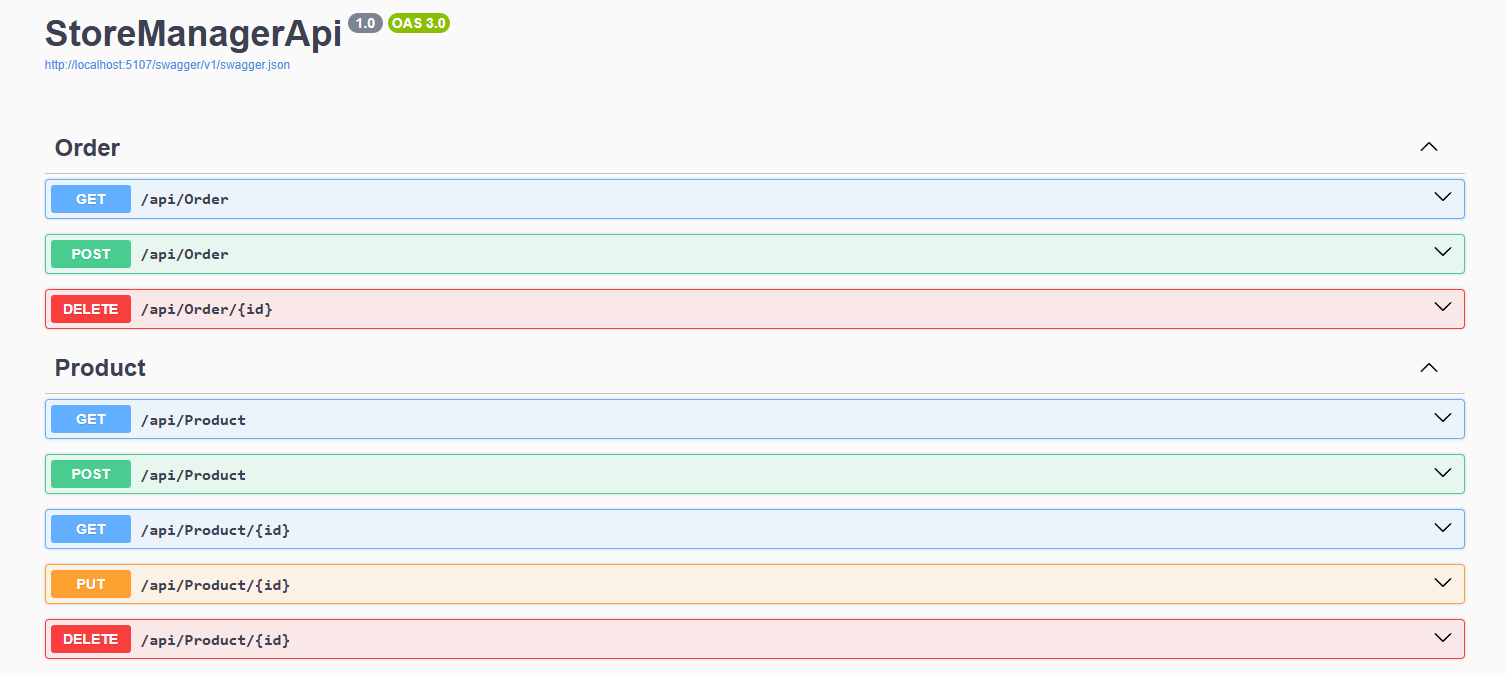
\includegraphics[width=0.8\textwidth]{fig/Рисунок_5_1.png}
	\caption{Страница тестирования API Swagger UI.}
	\label{fig:swagger_ui}
\end{figure}

\noindent \textcolor{CtpRed}{Внимание:} В случае ошибки "Подключение не защищено" / "NET::ERR\_CERT\_INVALID", в Visual Studio рядом с кнопкой запуска выберите http-профиль вместо https.

\noindent Далее необходимо протестировать методы GET и POST. С помощью метода POST можно добавить новые товары в базу данных. Для этого в разделе \texttt{Product} рядом с методом POST нажмите на <<стрелку>> и в открывшейся вкладке кнопку <<Try it out>>.

\begin{figure}[H]
	\centering
	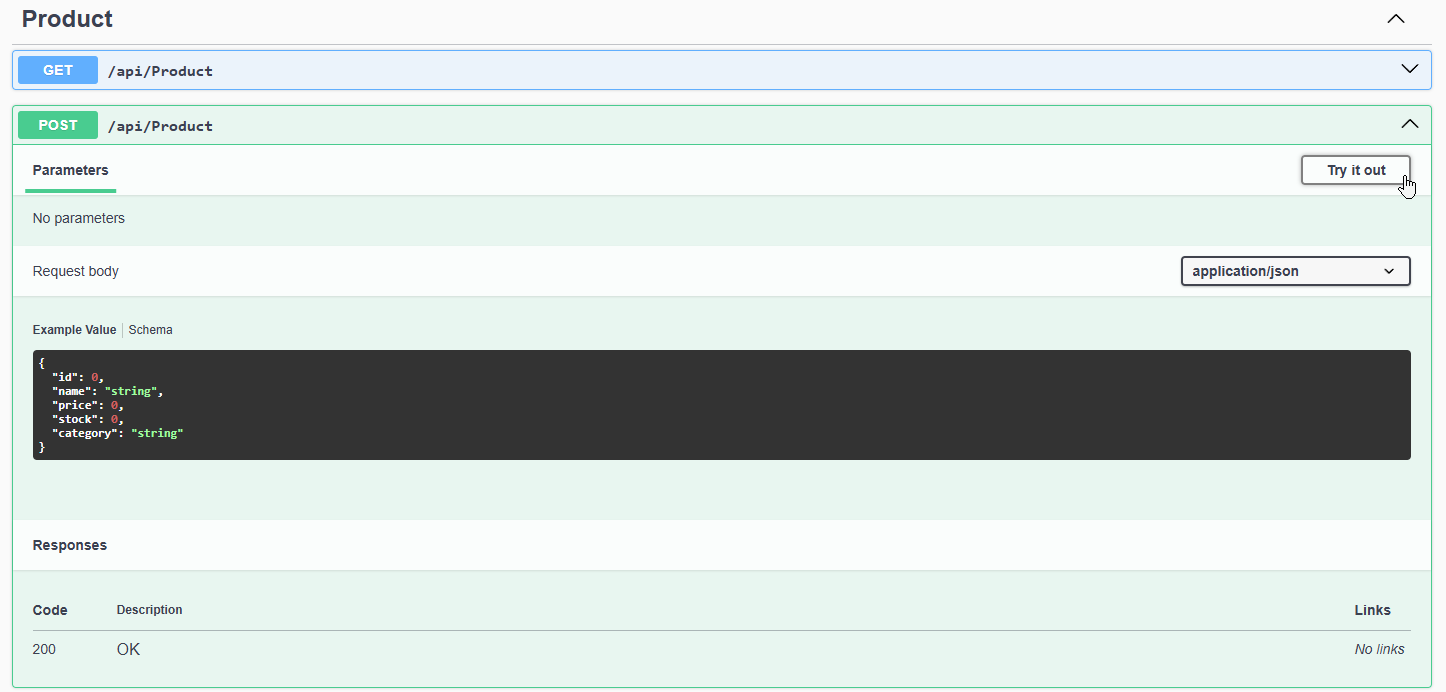
\includegraphics[width=0.8\textwidth]{fig/Рисунок_5_2.png}
	\caption{Меню метода POST в Swagger UI для контроллера Product.}
\end{figure}

\noindent В открывшемся окне необходимо изменить данные JSON-объекта на требующиеся и нажать кнопку <<Execute>>.

\begin{figure}[H]
	\centering
	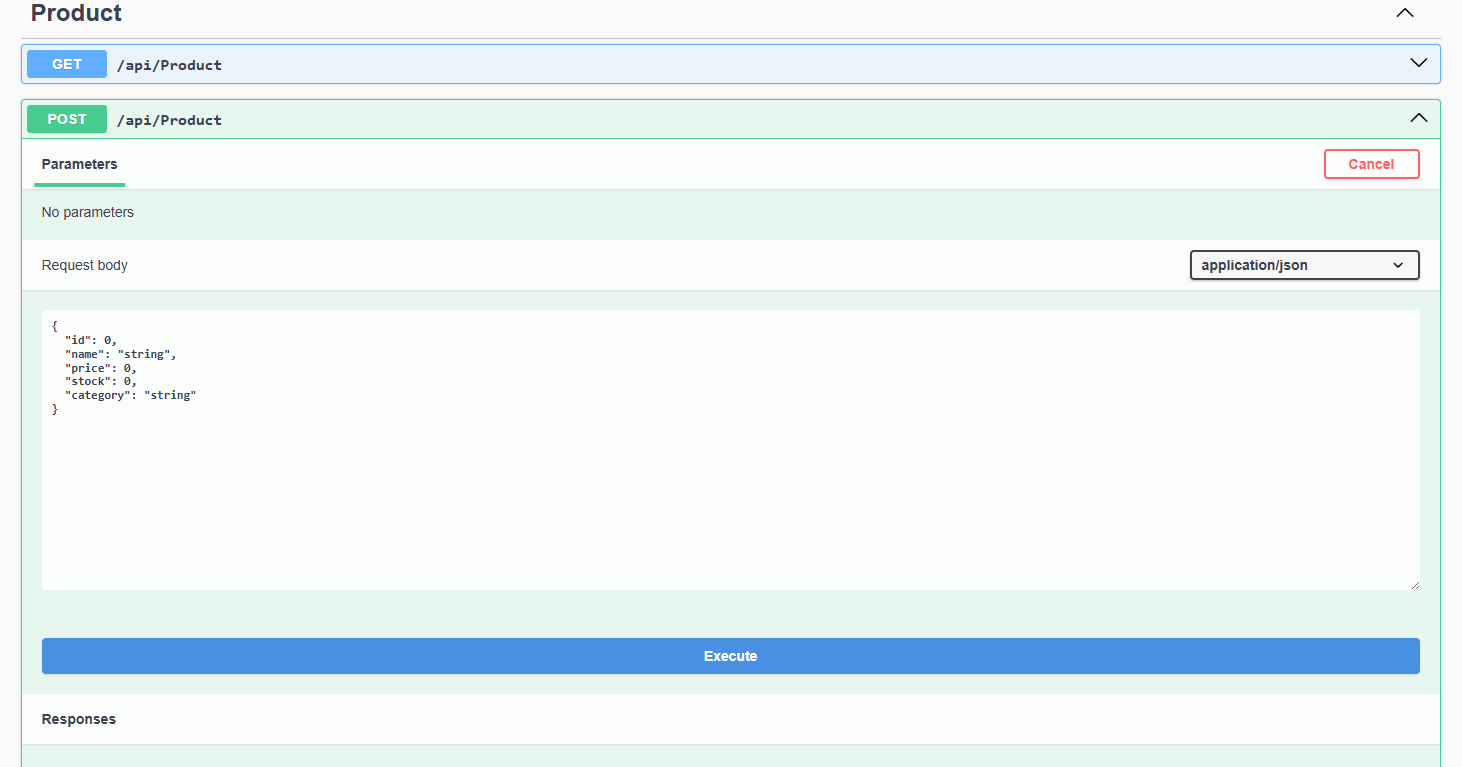
\includegraphics[width=0.8\textwidth]{fig/Рисунок_5_3.png}
	\caption{Добавление данных с помощью метода POST в Swagger UI.}
\end{figure}

\noindent Пример 1: POST — Добавление товара №1
\begin{code}
	\begin{minted}{json}
{
  "id": 0, // id будет присвоен автоматически базой данных
  "name": "Монитор Samsung",
  "price": 25000,
  "stock": 30,
  "category": "Мониторы и дисплеи"
}
\end{minted}
	\captionof{listing}{Пример JSON для POST запроса (Товар 1)}
\end{code}

\noindent Пример 2: POST — Добавление товара №2
\begin{code}
	\begin{minted}{json}
{
  "id": 0, // id будет присвоен автоматически базой данных
  "name": "Компьютерная мышь Logitech",
  "price": 25.99,
  "stock": 10,
  "category": "Периферия"
}
\end{minted}
	\captionof{listing}{Пример JSON для POST запроса (Товар 2)}
\end{code}

\noindent Далее аналогичным образом можно получить данные из базы данных с помощью метода GET. Для этого в разделе \texttt{GET /api/Product} необходимо нажать кнопку <<Try it out>>. В результате на экран будет выведен результат GET-запроса.

\begin{figure}[H]
	\centering
	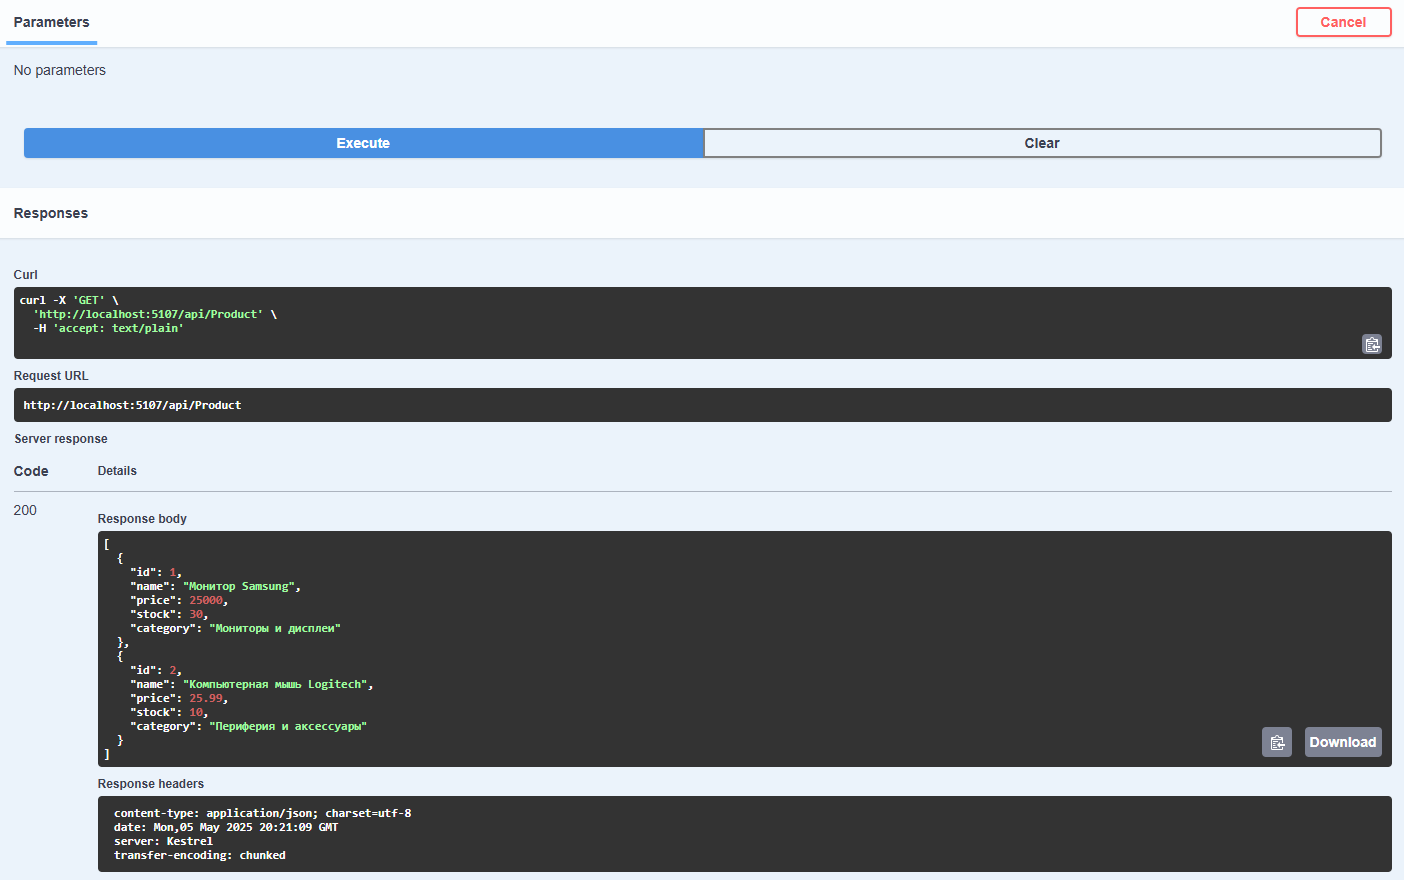
\includegraphics[width=0.8\textwidth]{fig/Рисунок_5_4.png}
	\caption{Выполнение запроса GET /api/Product и его результат в Swagger UI.}
\end{figure}

\noindent Пример ответа на GET-запрос:
\begin{code}
	\begin{minted}{json}
[
  {
    "id": 1,
    "name": "Монитор Samsung",
    "price": 25000,
    "stock": 30,
    "category": "Мониторы и дисплеи"
  },
  {
    "id": 2,
    "name": "Компьютерная мышь Logitech",
    "price": 25.99,
    "stock": 10,
    "category": "Периферия"
  }
]
\end{minted}
	\captionof{listing}{Пример ответа на GET /api/Product}
\end{code}
\noindent \textcolor{CtpRed}{Внимание:} если вы столкнулись с тем, что новые изменения, которые вы вносите в приложение не работают или не дают нужного результата (программа выдает ошибку 401, 500 и т.д.) необходимо удалить файл базы данных \texttt{store.db}. Программа автоматически создаст файл заново, вам нужно будет только добавить новые товары через интерфейс приложения WPF (или Swagger UI для API).

\pagebreak

\section{Контрольные вопросы~\texorpdfstring{\iicon{}}{}}
\begin{enumerate}
	\item \textbf{Что такое ASP.NET Core Web API и для чего он используется?} \\
	      ASP.NET Core Web API — это фреймворк для создания HTTP-сервисов, которые могут быть доступны различным клиентам (веб-браузеры, мобильные приложения и др.). Он используется для построения RESTful API, предоставляющих доступ к данным и бизнес-логике приложения.

	\item \textbf{Какую роль выполняет файл \texttt{Program.cs} в ASP.NET Core приложении?} \\
	      Файл \texttt{Program.cs} является точкой входа приложения. Он отвечает за конфигурацию сервисов приложения (включая внедрение зависимостей, например, \texttt{DbContext}), настройку конвейера обработки HTTP-запросов (middleware), определение источников конфигурации и запуск веб-сервера.

	\item \textbf{Что такое модель (Model) в контексте EF Core и ASP.NET Core? Приведите пример из лабораторной работы.} \\
	      Модель представляет структуру данных, с которыми работает приложение. В EF Core модель обычно соответствует таблице в базе данных. В ASP.NET Core модели также используются для передачи данных между контроллером и клиентом. Пример из работы: класс \texttt{Product} с свойствами \texttt{Id}, \texttt{Name}, \texttt{Price}, \texttt{Stock}, \texttt{Category}.

	\item \textbf{Объясните назначение класса \texttt{DbContext} (на примере \texttt{StoreDbContext}) в Entity Framework Core.} \\
	      Класс \texttt{DbContext} (например, \texttt{StoreDbContext}) представляет сессию с базой данных и позволяет запрашивать и сохранять данные. Он содержит свойства типа \texttt{DbSet<TEntity>} для каждой сущности (таблицы) в модели. В методе \texttt{OnConfiguring} настраивается подключение к БД, а в \texttt{OnModelCreating} — детали модели данных, такие как связи и ограничения.

	\item \textbf{Что такое контроллер в ASP.NET Core Web API (на примере \texttt{ProductController})? Какие задачи он решает?} \\
	      Контроллер — это класс, который обрабатывает входящие HTTP-запросы, выполняет соответствующую бизнес-логику (часто взаимодействуя с моделями, сервисами и \texttt{DbContext}) и возвращает HTTP-ответы. \texttt{ProductController} в данной работе управляет операциями CRUD (создание, чтение, обновление, удаление) для сущностей товаров.

	\item \textbf{Какие HTTP-методы были реализованы в \texttt{ProductController} и каково их стандартное назначение в REST API?} \\
	      Были реализованы:
	      \begin{itemize}
		      \item \texttt{GET}: для получения ресурсов (всех товаров или одного товара по его идентификатору).
		      \item \texttt{POST}: для создания нового ресурса (нового товара).
		      \item \texttt{PUT}: для полного обновления существующего ресурса (обновления информации о товаре).
		      \item \texttt{DELETE}: для удаления ресурса (удаления товара по его идентификатору).
	      \end{itemize}

	\item \textbf{Что такое Swagger (OpenAPI) и для чего он использовался в лабораторной работе?} \\
	      Swagger (реализация спецификации OpenAPI) — это набор инструментов для проектирования, создания, документирования и использования RESTful веб-сервисов. В лабораторной работе он использовался для автоматической генерации интерактивной документации API, которая позволяет просматривать доступные эндпоинты, их параметры, типы возвращаемых данных и тестировать их непосредственно из браузера.

	\item \textbf{Как в \texttt{Program.cs} была настроена работа с базой данных SQLite и её автоматическое создание?} \\
	      Работа с SQLite была настроена путем регистрации \texttt{StoreDbContext} в контейнере зависимостей с помощью метода \texttt{builder.Services.AddDbContext<StoreDbContext>(options => options.Use\-Sqlite("Data Source=store.db"));}. Автоматическое создание базы данных (если она не существует) при запуске приложения обеспечивалось вызовом \texttt{db.Database.Ensure\-Created();} внутри блока, получающего сервис \texttt{StoreDbContext} из провайдера сервисов.

	\item \textbf{Объясните принцип маршрутизации в ASP.NET Core Web API на примере \texttt{Product\-Controller}.} \\
	      Маршрутизация определяет, как HTTP-запросы сопоставляются с методами действий контроллера. Атрибут \texttt{[ApiController]} на классе контроллера активирует стандартное поведение для API. Атрибут \texttt{[Route("api/[controller]")]} на \texttt{ProductController} задает базовый маршрут как \texttt{/api/Product}. Далее, атрибуты HTTP-методов (\texttt{[HttpGet]}, \texttt{[HttpPost]}, \texttt{[HttpGet("{id}")]} и т.д.) на методах действий уточняют путь и HTTP-метод для каждого эндпоинта. Например, \texttt{[HttpGet("{id}")]} на методе \texttt{Get(int id)} означает, что запрос \texttt{GET /api/Pro\-duct/5} будет обработан этим методом.

	\item \textbf{В чем заключается механизм Dependency Injection (DI), использованный в конструкторе \texttt{ProductController(StoreDbContext context)}?} \\
	      Dependency Injection (внедрение зависимостей) — это паттерн проектирования, при котором зависимости объекта (например, экземпляр \texttt{StoreDbContext} для \texttt{ProductController}) предоставляются ему извне (обычно контейнером DI), а не создаются им самим. В \texttt{Program.cs} \texttt{StoreDbContext} регистрируется как сервис. Когда ASP.NET Core создает экземпляр \texttt{Product\-Controller}, контейнер DI автоматически <<внедряет>> (передает) зарегистрированный экземпляр \texttt{StoreDbContext} в его конструктор. Это способствует слабой связанности компонентов и улучшает тестируемость.
\end{enumerate}

\end{document}
